\documentclass{article}

\usepackage{graphicx}
\usepackage[margin=1in]{geometry}
\usepackage{enumitem}
\usepackage{booktabs}
\usepackage{float}

\begin{document}

\title{Multi-config experiment report}
\author{}
\date{27 January 2026}
\maketitle

\section*{Overview}
This report summarizes the controlled experiments with various configuration for kernels. All runs are logistic models with different kernel counts and selection method.

\section*{Run configuration}
Common settings: topM=300, response\_fn=abs\_max, batch size 64, lr=5e-4, epochs=60.

\subsection*{MMR runs}

\begin{center}
\begin{tabular}{llllll}
\toprule
Run & Model & K & topM & std\_feat & std\_resp \\
\midrule
exp\_022\_mmr & logistic & 3 & 300 & False & False \\
exp\_023\_mmr & logistic & 5 & 300 & False & False \\
exp\_024\_mmr & logistic & 200 & 300 & False & False \\
exp\_025\_mmr & logistic & 300 & 300 & False & False \\
\bottomrule
\end{tabular}
\end{center}

\subsection*{ABESS runs}
\begin{center}
\begin{tabular}{llllll}
\toprule
Run & Model & K & topM & std\_feat & std\_resp \\
\midrule
exp\_029\_abess & logistic & 3 & 300 & False & False \\
exp\_030\_abess & logistic & 5 & 300 & False & False \\
exp\_031\_abess & logistic & 200 & 300 & False & False \\
exp\_032\_abess & logistic & 300 & 300 & False & False \\
\bottomrule
\end{tabular}
\end{center}

\section*{Validation/Test metrics}
\subsection*{MMR runs}
\begin{center}
\begin{tabular}{lccccc}
\toprule
Run & Val AUC & Val ACC & Test AUC & Test ACC & Intercept \\
\midrule
\texttt{exp\_022\_mmr} & 0.9085 & 0.8011 & 0.9239 & 0.7914 & -0.691 \\
\texttt{exp\_023\_mmr} & 0.9071 & 0.7765 & 0.9234 & 0.7594 & -0.908 \\
\texttt{exp\_024\_mmr} & 0.9047 & 0.8156 & 0.9180 & 0.7909 & -1.215 \\
\texttt{exp\_025\_mmr} & 0.8790 & 0.8006 & 0.8927 & 0.8182 & -1.204 \\
\bottomrule
\end{tabular}
\end{center}

\subsection*{ABESS runs}
\begin{center}
\begin{tabular}{lccccc}
\toprule
Run & Val AUC & Val ACC & Test AUC & Test ACC & Intercept \\
\midrule
\texttt{exp\_029\_abess} & 0.9059 & 0.7615 & 0.9216 & 0.7455 & -0.649 \\
\texttt{exp\_030\_abess} & 0.9075 & 0.7838 & 0.9225 & 0.7684 & -1.004 \\
\texttt{exp\_031\_abess} & 0.9095 & 0.7849 & 0.9236 & 0.7690 & -1.267 \\
\texttt{exp\_032\_abess} & 0.8824 & 0.8028 & 0.8966 & 0.8032 & -1.224 \\
\bottomrule
\end{tabular}
\end{center}

\clearpage
\section*{Heatmap comparisons}
\subsection*{MMR}
\begin{figure}[H]
    \centering
    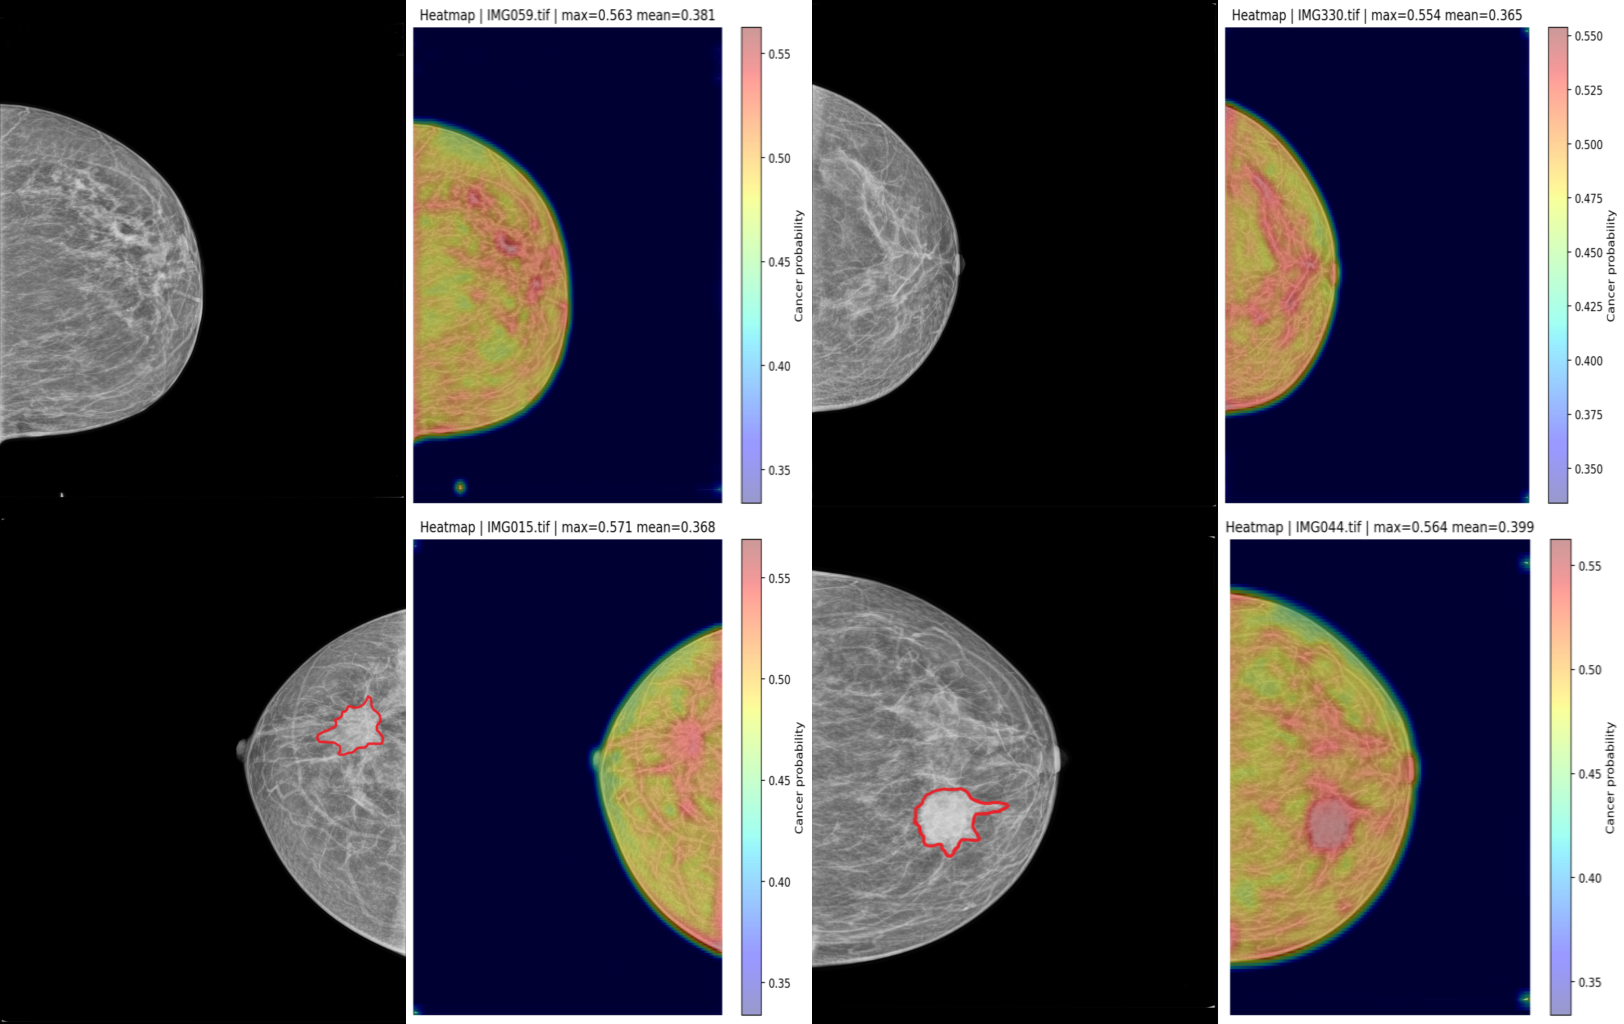
\includegraphics[width=0.95\linewidth]{../results/exp_022_mmr/heatmaps_side_by_side.png}
    \caption{MMR heatmaps for exp\_022 (2 normal + 2 malignant).}
\end{figure}
\begin{figure}[H]
    \centering
    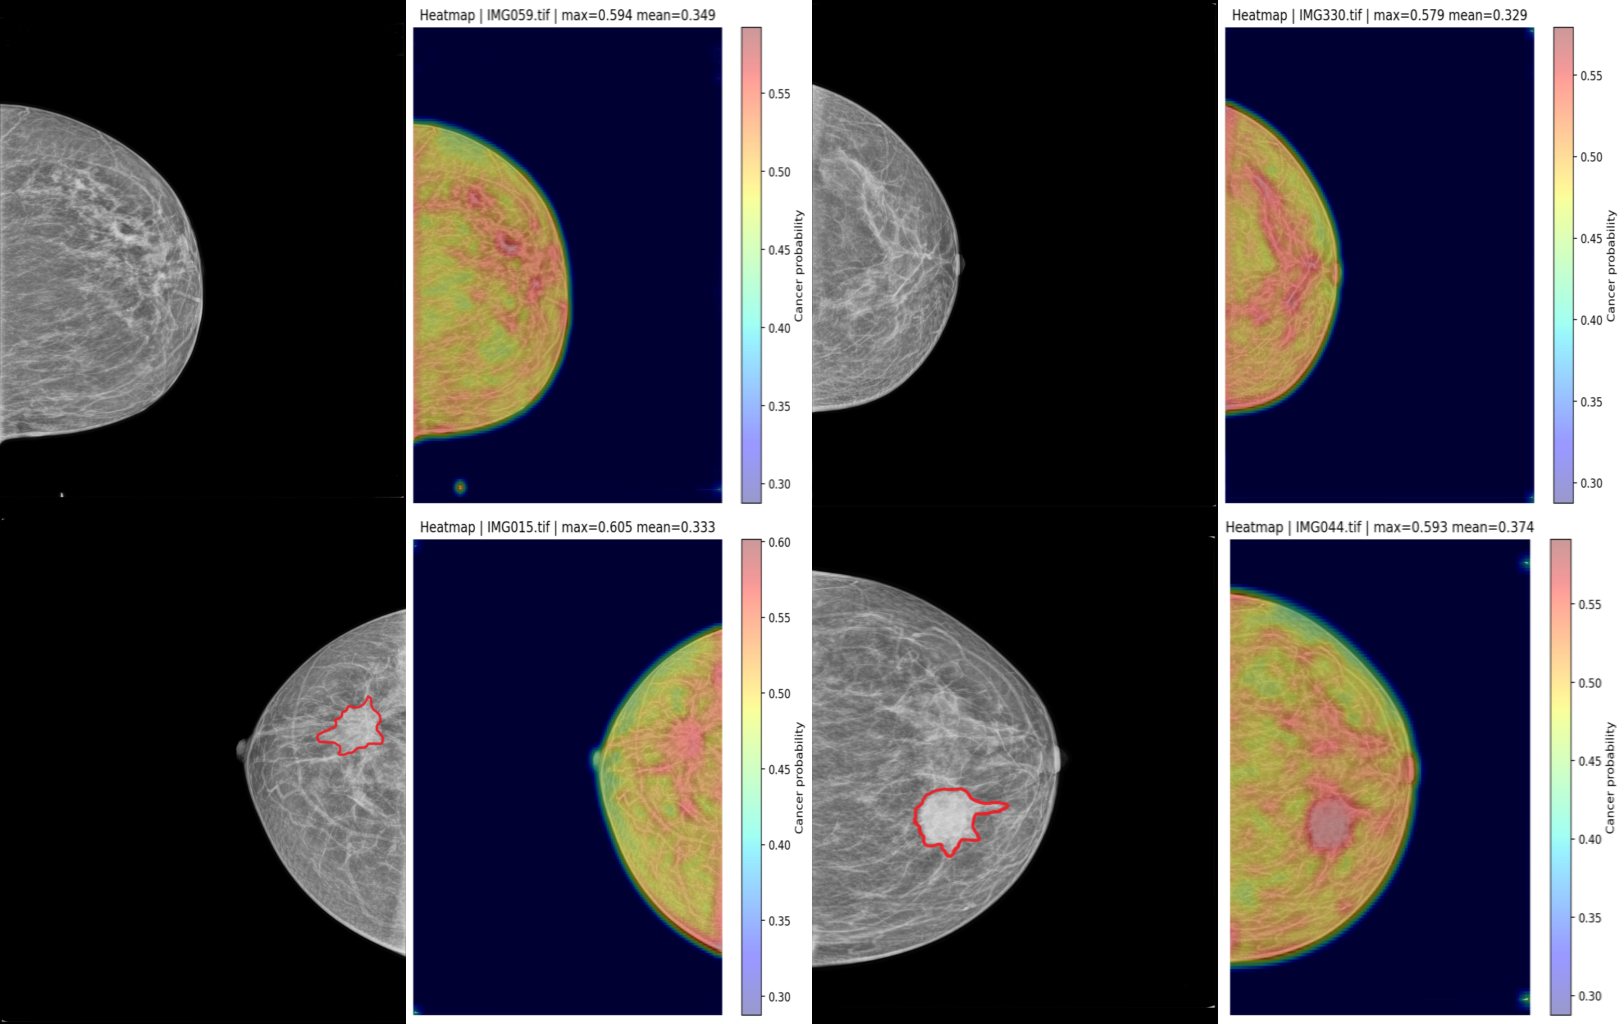
\includegraphics[width=0.95\linewidth]{../results/exp_023_mmr/heatmaps_side_by_side.png}
    \caption{MMR heatmaps for exp\_023 (2 normal + 2 malignant).}
\end{figure}
\begin{figure}[H]
    \centering
    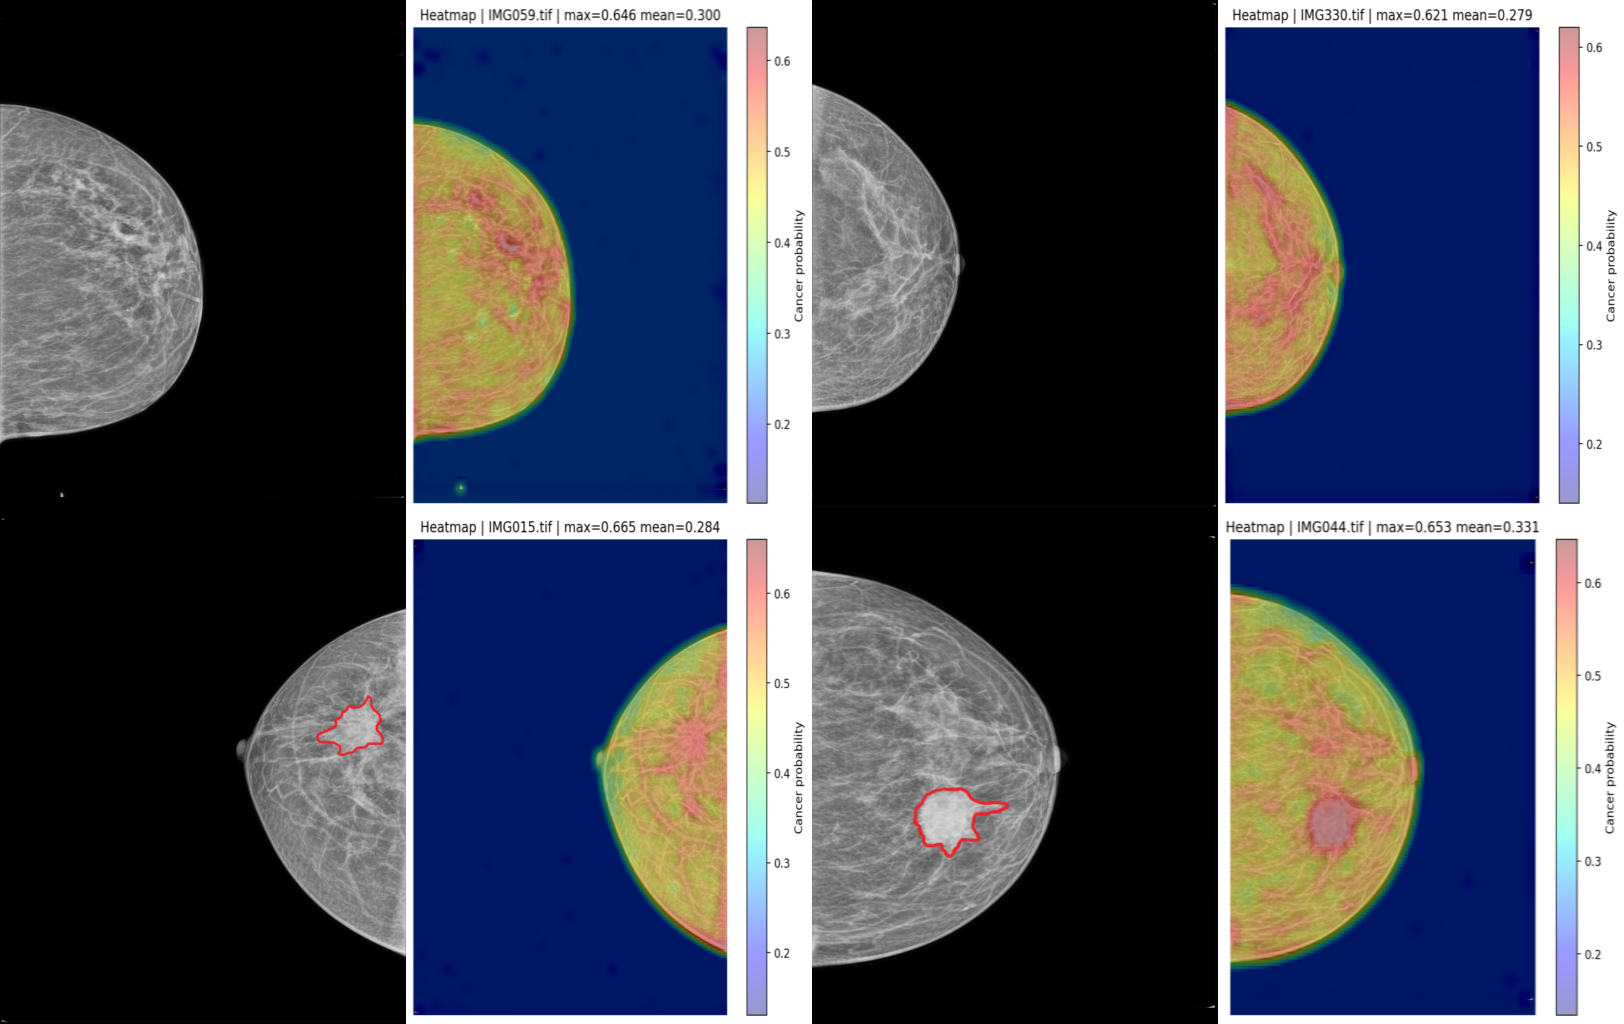
\includegraphics[width=0.95\linewidth]{../results/exp_024_mmr/heatmaps_side_by_side.png}
    \caption{MMR heatmaps for exp\_024 (2 normal + 2 malignant).}
\end{figure}
\begin{figure}[H]
    \centering
    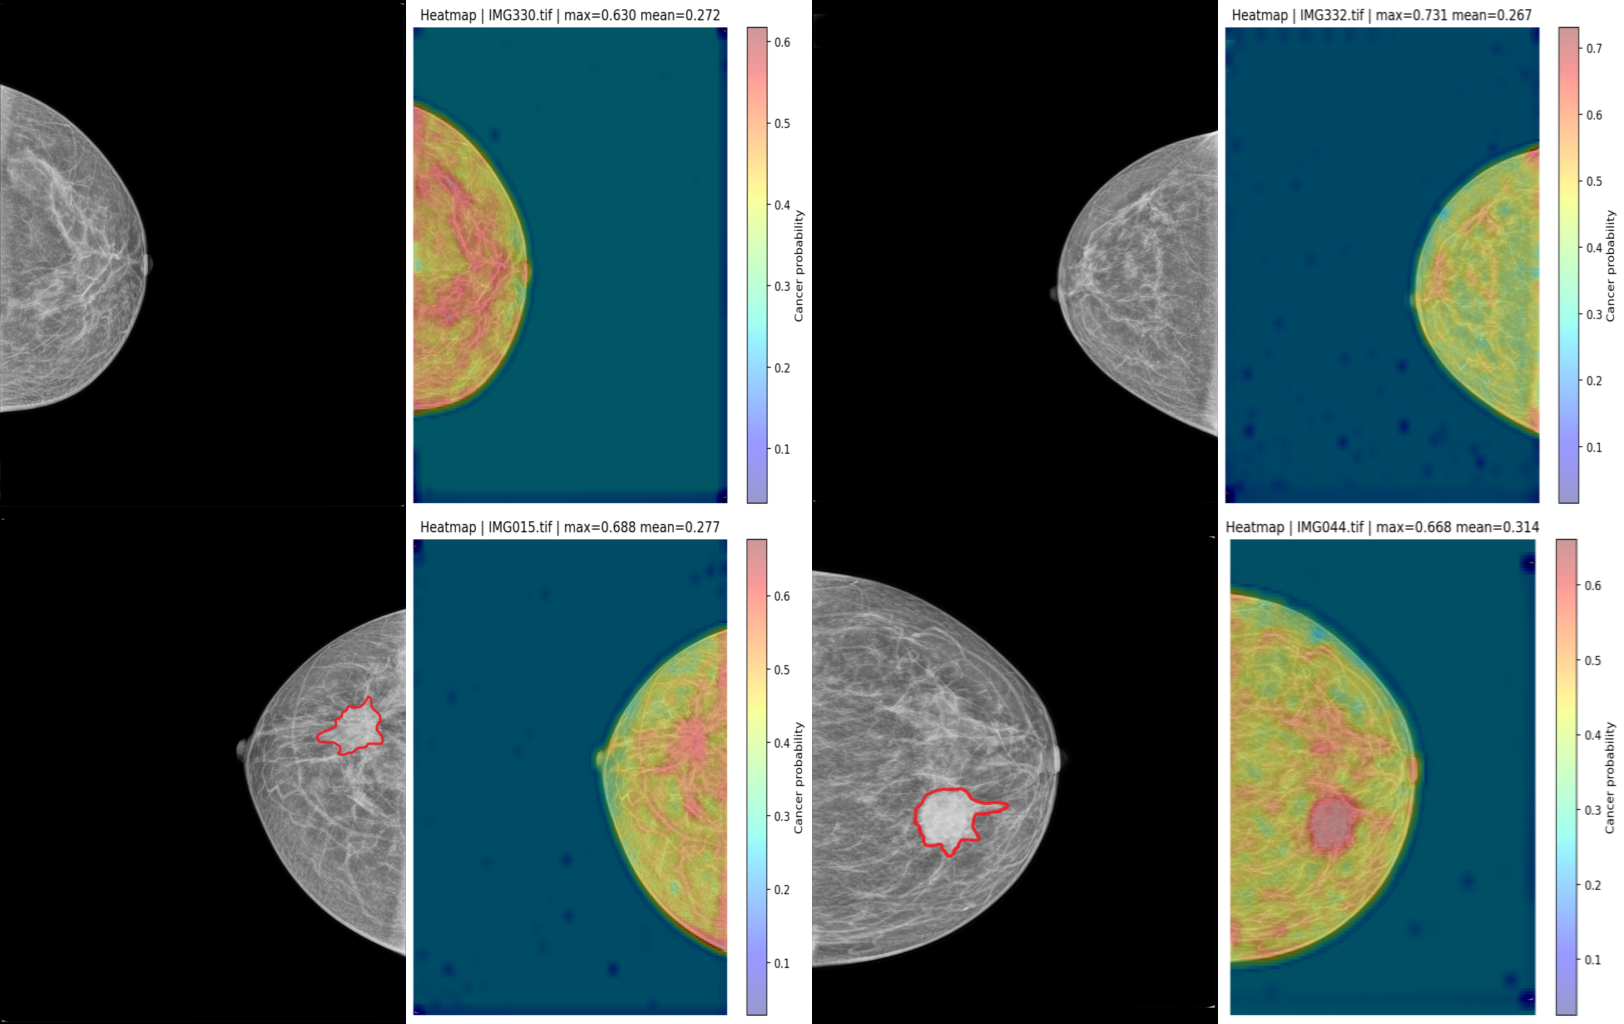
\includegraphics[width=0.95\linewidth]{../results/exp_025_mmr/heatmaps_side_by_side.png}
    \caption{MMR heatmaps for exp\_025 (2 normal + 2 malignant).}
\end{figure}

\subsection*{ABESS}
\begin{figure}[H]
    \centering
    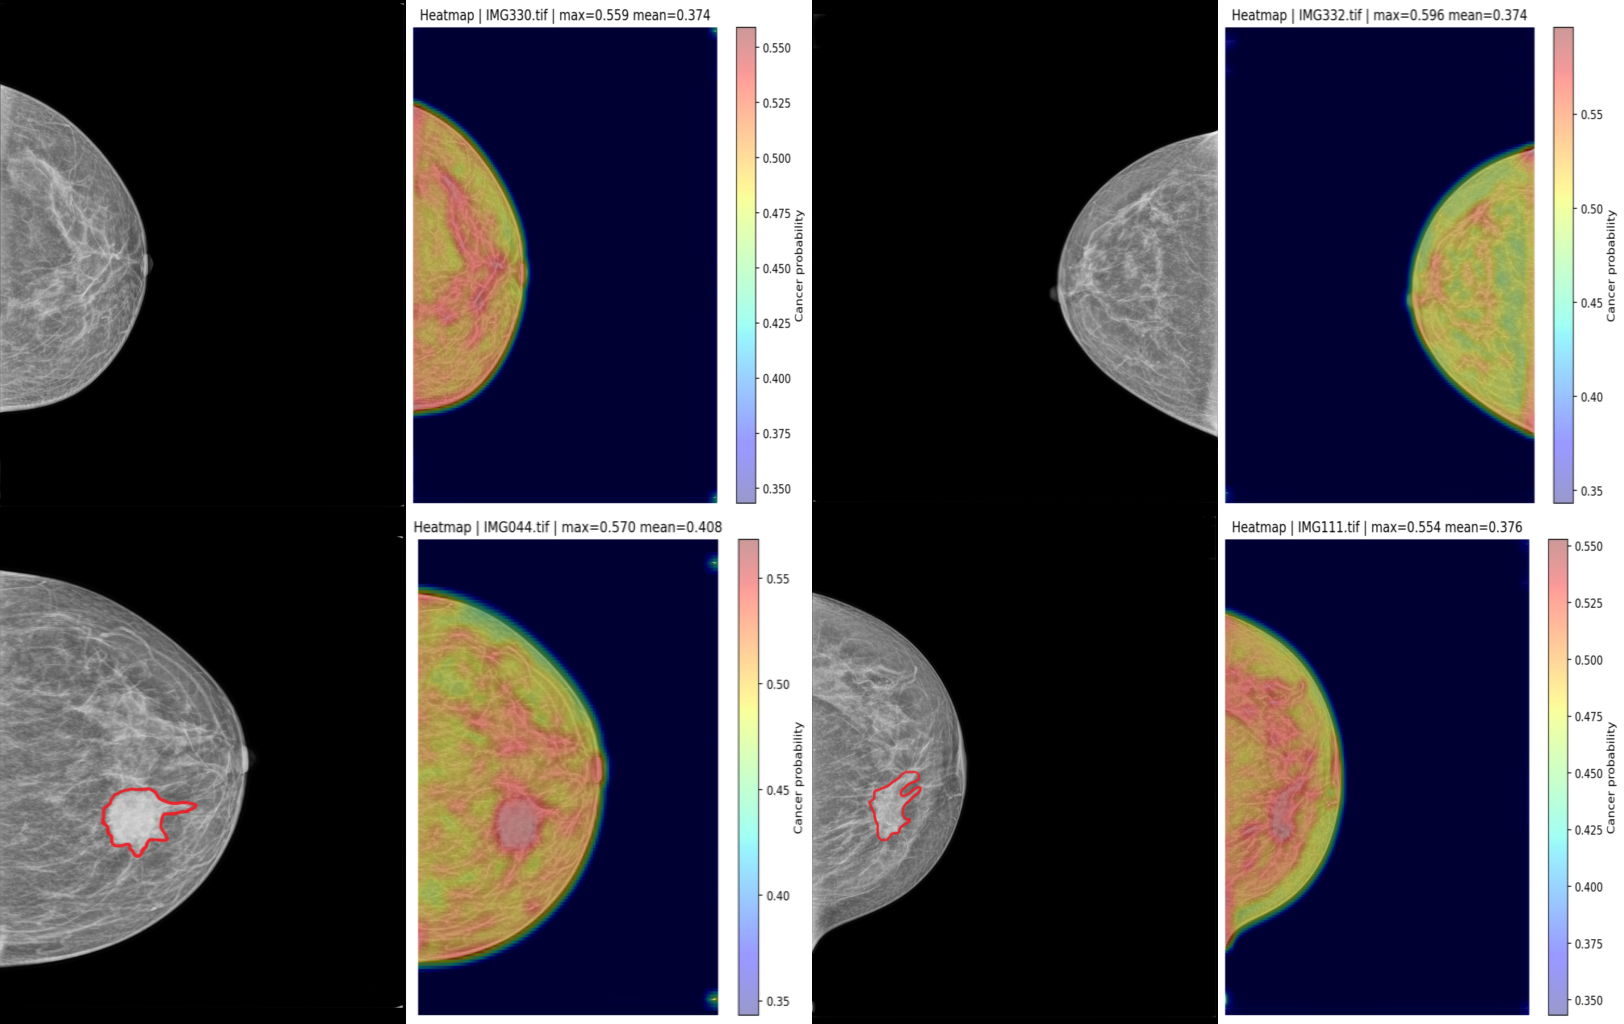
\includegraphics[width=0.95\linewidth]{../results/exp_029_abess/heatmaps_side_by_side.png}
    \caption{ABESS heatmaps for exp\_029 (2 normal + 2 malignant).}
\end{figure}
\begin{figure}[H]
    \centering
    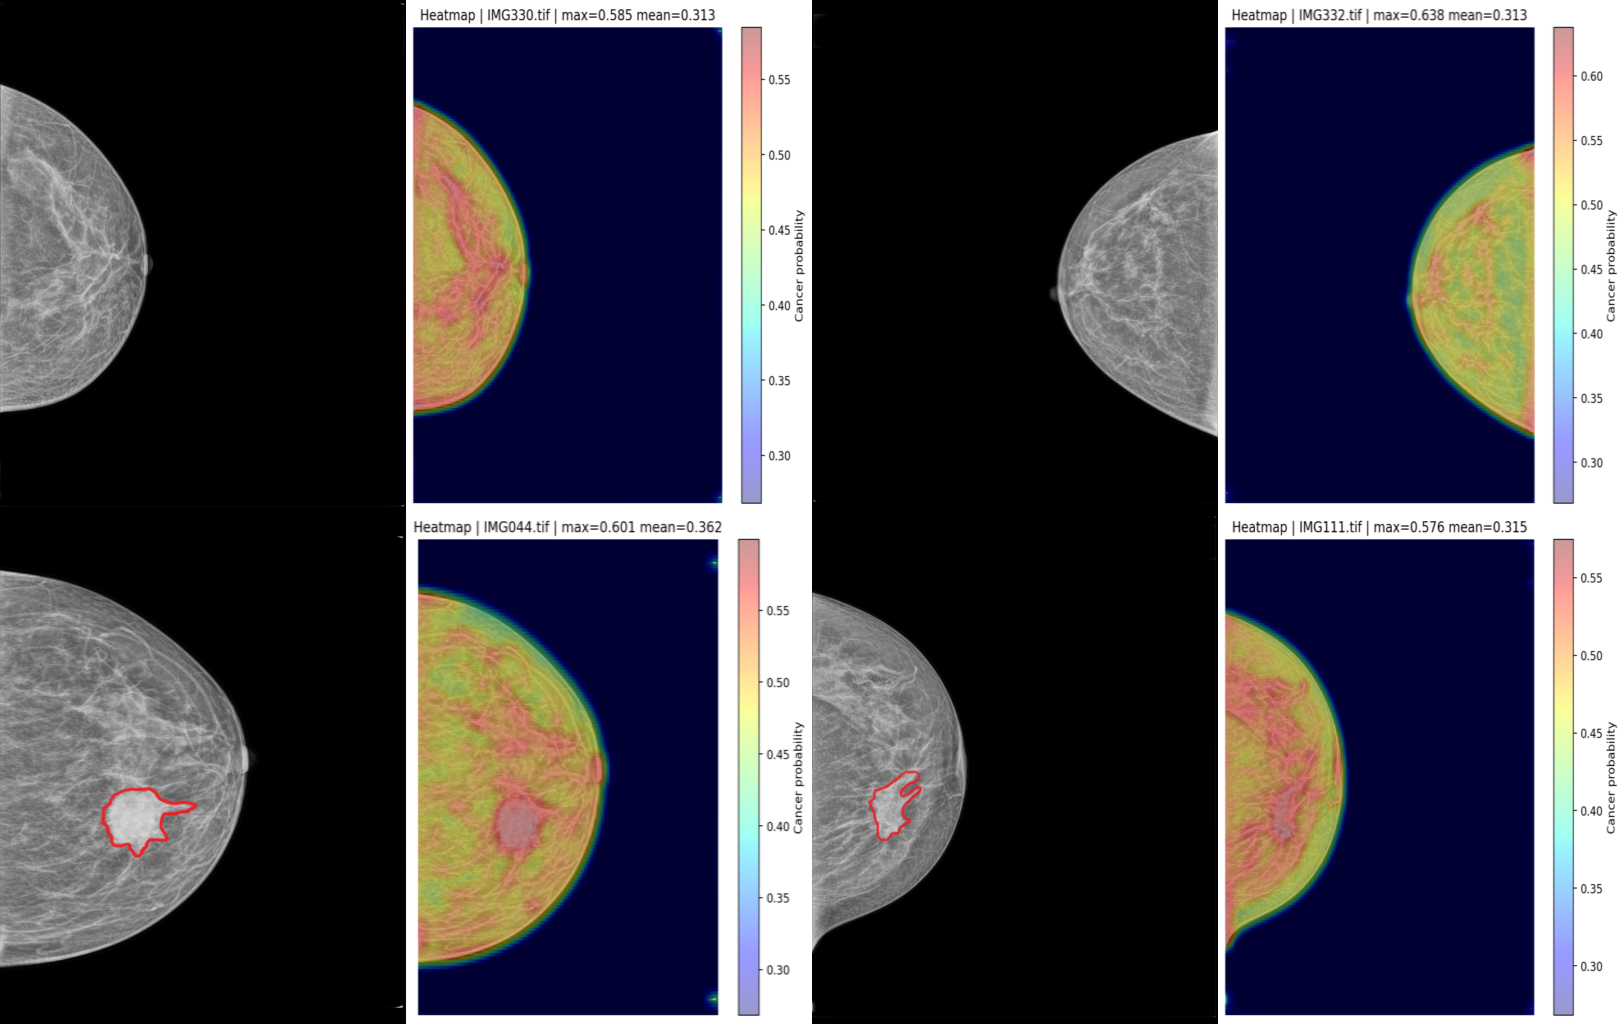
\includegraphics[width=0.95\linewidth]{../results/exp_030_abess/heatmaps_side_by_side.png}
    \caption{ABESS heatmaps for exp\_030 (2 normal + 2 malignant).}
\end{figure}
\begin{figure}[H]
    \centering
    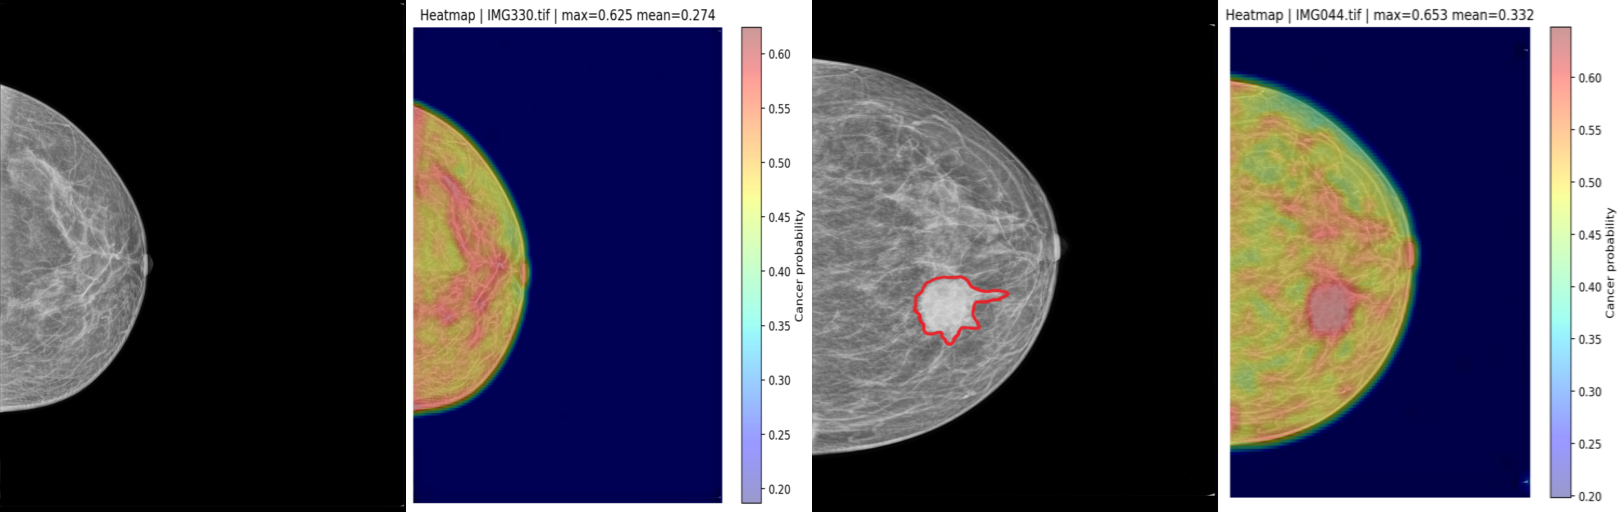
\includegraphics[width=0.95\linewidth]{../results/exp_031_abess/heatmaps_side_by_side.png}
    \caption{ABESS heatmaps for exp\_031 (partial set available).}
\end{figure}

\section*{Summary}
Across MMR runs, test AUC is highest for exp\_022\_mmr (0.9239), while test accuracy peaks at exp\_025\_mmr (0.8182).  
Across ABESS runs, exp\_031\_abess achieves the best test AUC (0.9236), and exp\_032\_abess has the best test accuracy (0.8032).  
Overall, MMR runs show slightly higher peak AUC/ACC than ABESS in these settings.

\section*{Conclusion}
If prioritizing test AUC, exp\_022\_mmr is the best overall.  
If prioritizing test accuracy, exp\_025\_mmr is the best overall.  
Among ABESS configurations, exp\_031\_abess (AUC) and exp\_032\_abess (ACC) are the strongest.

\section*{Summary plot}
\begin{figure}[H]
    \centering
    \includegraphics[width=0.95\linewidth]{../results/multi_config_summary.png}
    \caption{AUC and accuracy for validation/test across multi-config runs.}
    \label{fig:multi_config_summary}
\end{figure}


\clearpage
\section*{Additional MMR variants (n\_per\_family / K)}
\begin{center}
\begin{tabular}{lcccccc}
\toprule
Run & n\_per\_family & K & topM & Val AUC & Test AUC & Test ACC \\
\midrule
exp\_022\_mmr\_n1\_k1 & 1 & 1 & 300 & 0.8994 & 0.9157 & 0.8449 \\
exp\_022\_mmr\_n3\_k1 & 3 & 1 & 300 & 0.9010 & 0.9179 & 0.8428 \\
exp\_022\_mmr\_n3\_k3 & 3 & 3 & 300 & 0.9085 & 0.9101 & 0.8417 \\
exp\_022\_mmr\_n10\_k3 & 10 & 3 & 65 & 0.9054 & 0.9032 & 0.8449 \\
\bottomrule
\end{tabular}
\end{center}

\paragraph{Summary}
These reduced-bank variants maintain strong test accuracy (around 0.84--0.85) but slightly trail the best baseline MMR AUCs.
Compared with the top-of-report baselines (exp\_022\_mmr AUC 0.9239, exp\_025\_mmr ACC 0.8182),
the n\_per\_family variants trade a small AUC drop for competitive accuracy.

\begin{figure}[H]
    \centering
    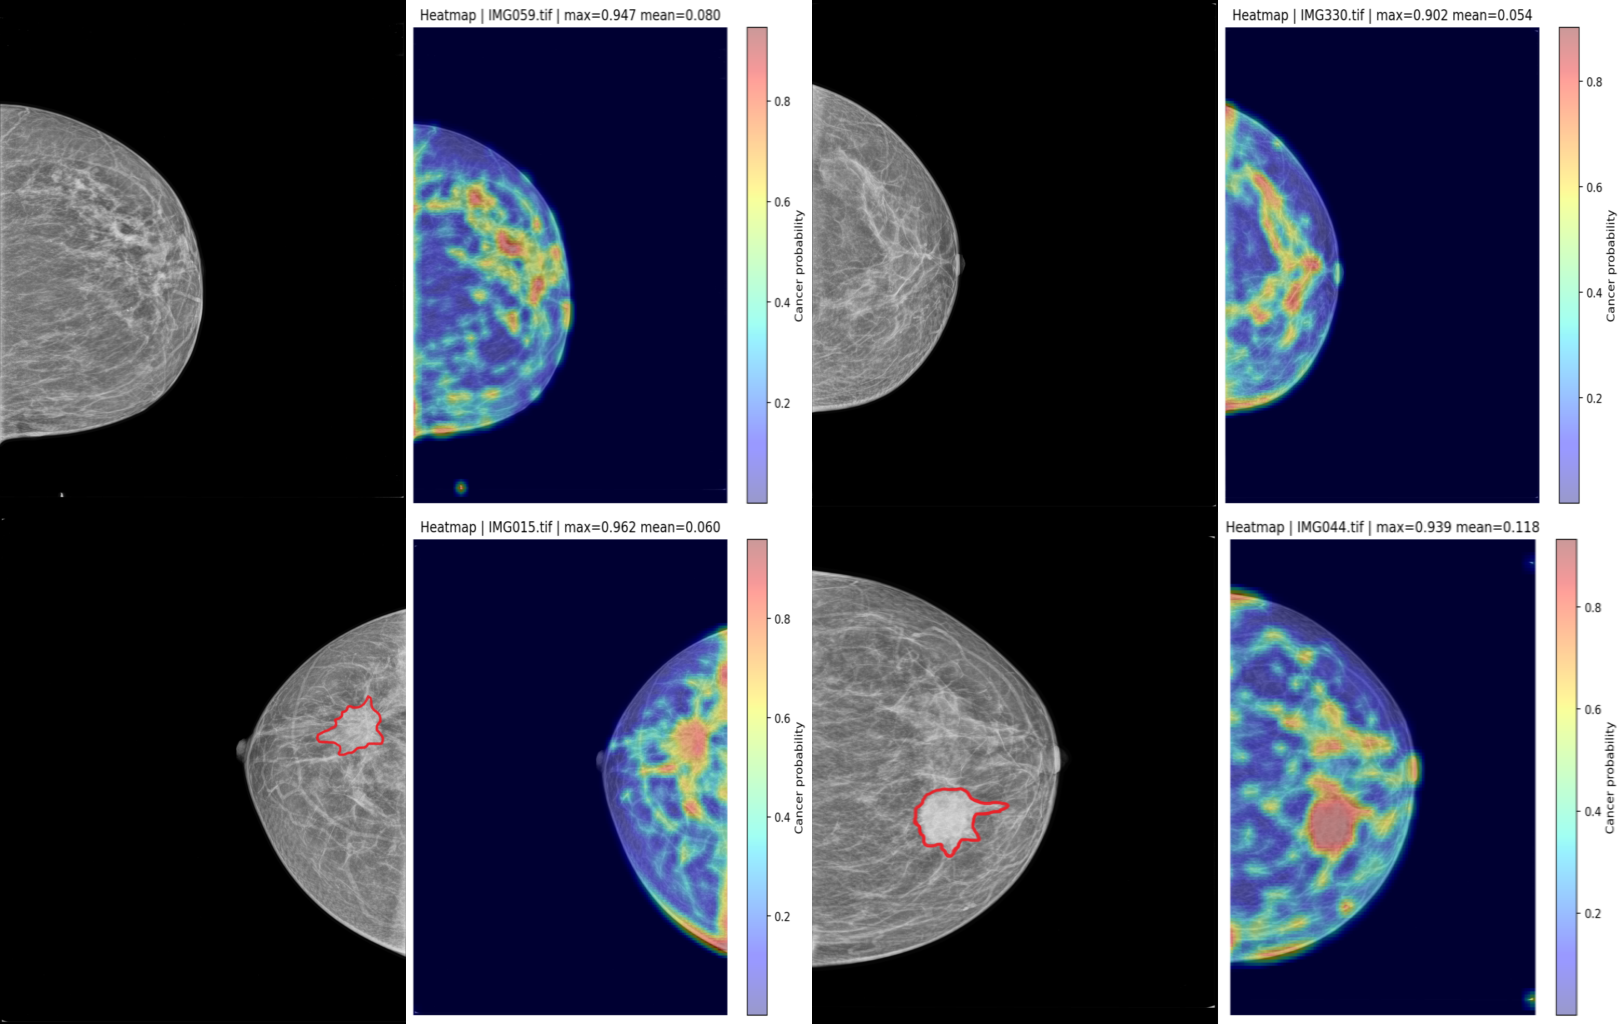
\includegraphics[width=0.95\linewidth]{../results/exp_022_mmr_n1_k1/heatmaps_side_by_side.png}
    \caption{Heatmaps for \texttt{exp\_022\_mmr\_n1\_k1}.}
\end{figure}
\begin{figure}[H]
    \centering
    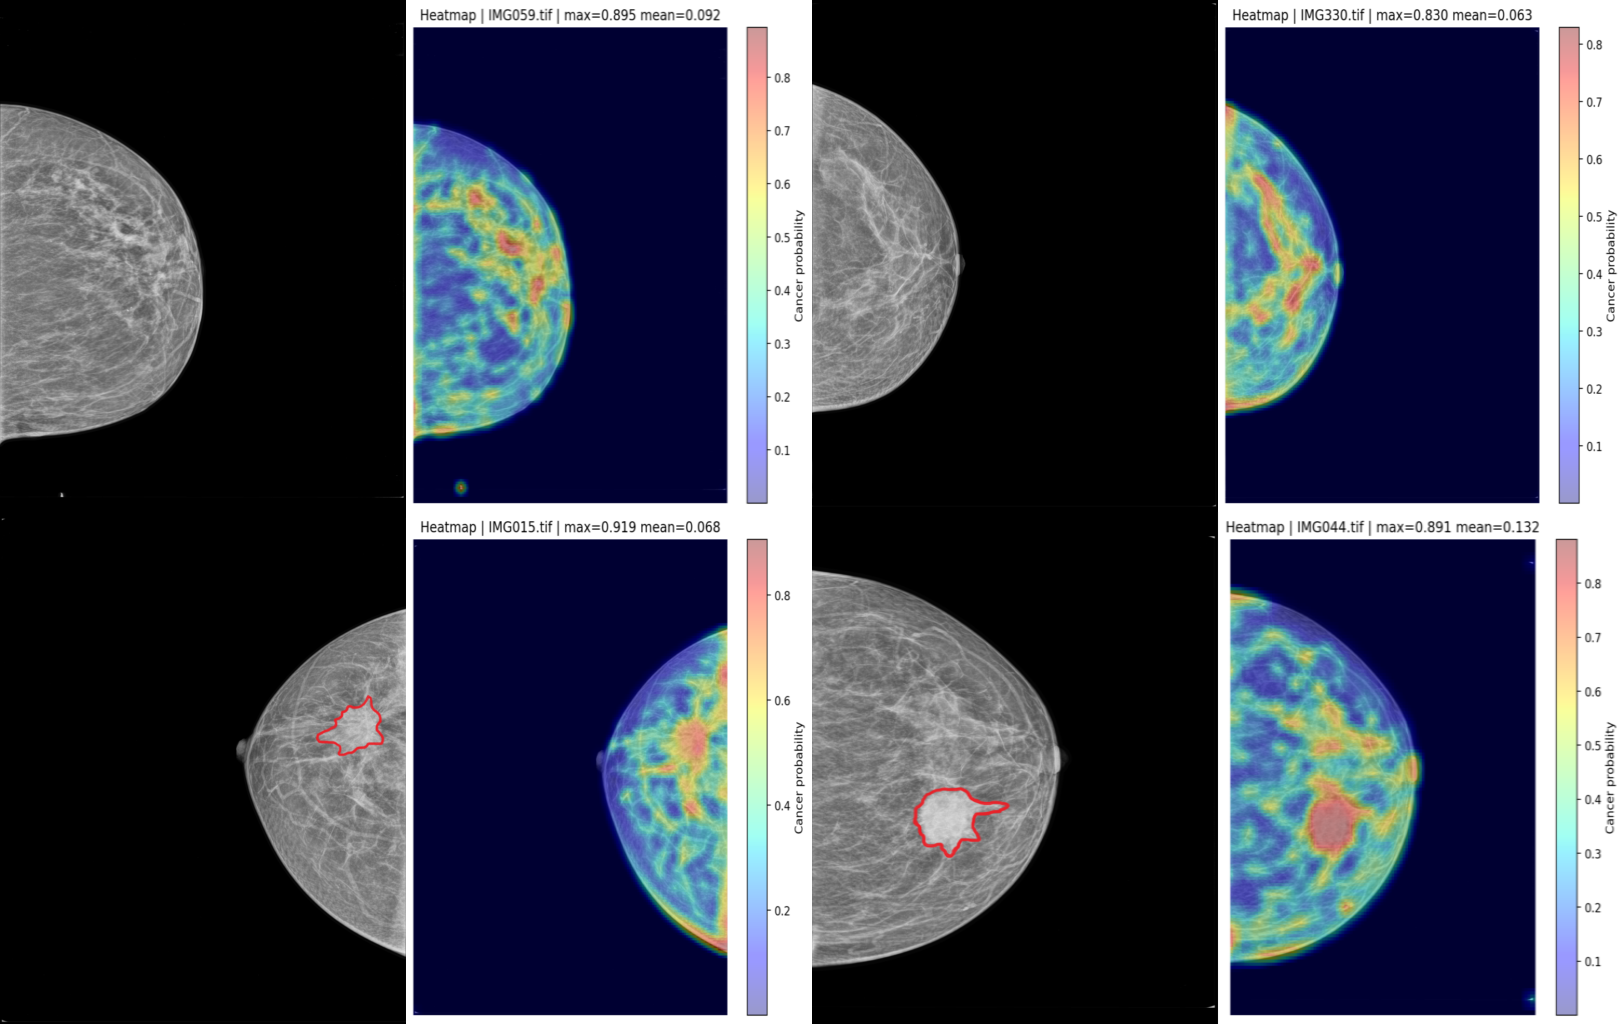
\includegraphics[width=0.95\linewidth]{../results/exp_022_mmr_n3_k1/heatmaps_side_by_side.png}
    \caption{Heatmaps for \texttt{exp\_022\_mmr\_n3\_k1}.}
\end{figure}
\begin{figure}[H]
    \centering
    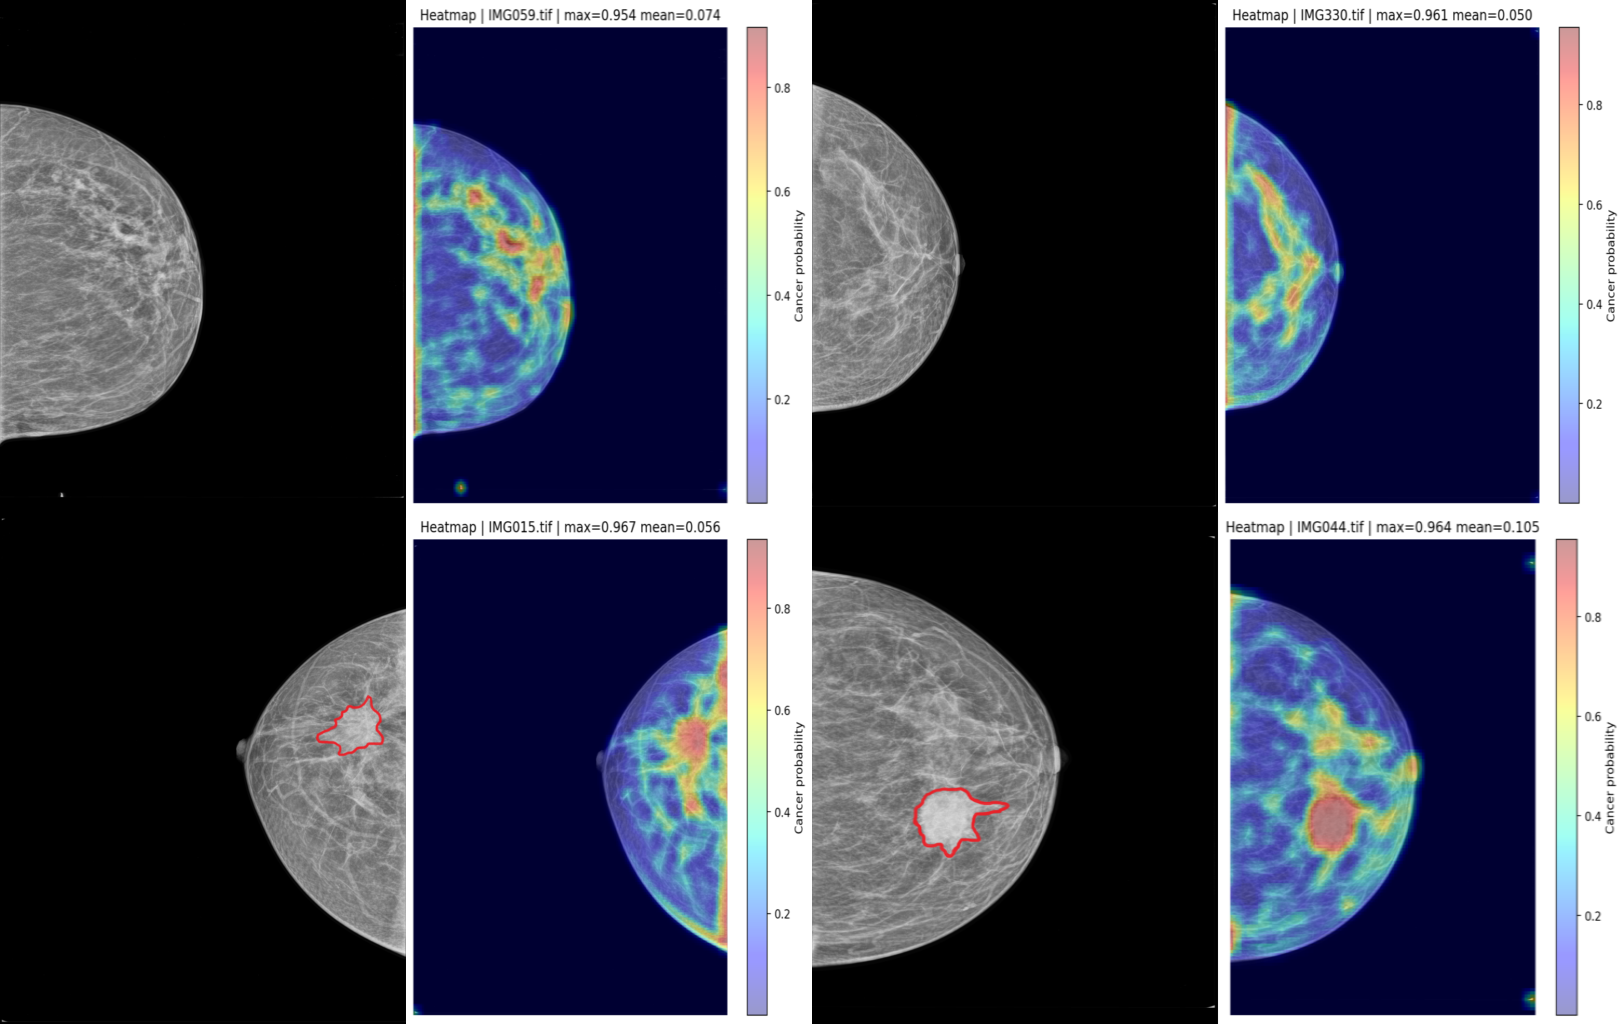
\includegraphics[width=0.95\linewidth]{../results/exp_022_mmr_n3_k3/heatmaps_side_by_side.png}
    \caption{Heatmaps for \texttt{exp\_022\_mmr\_n3\_k3}.}
\end{figure}
\begin{figure}[H]
    \centering
    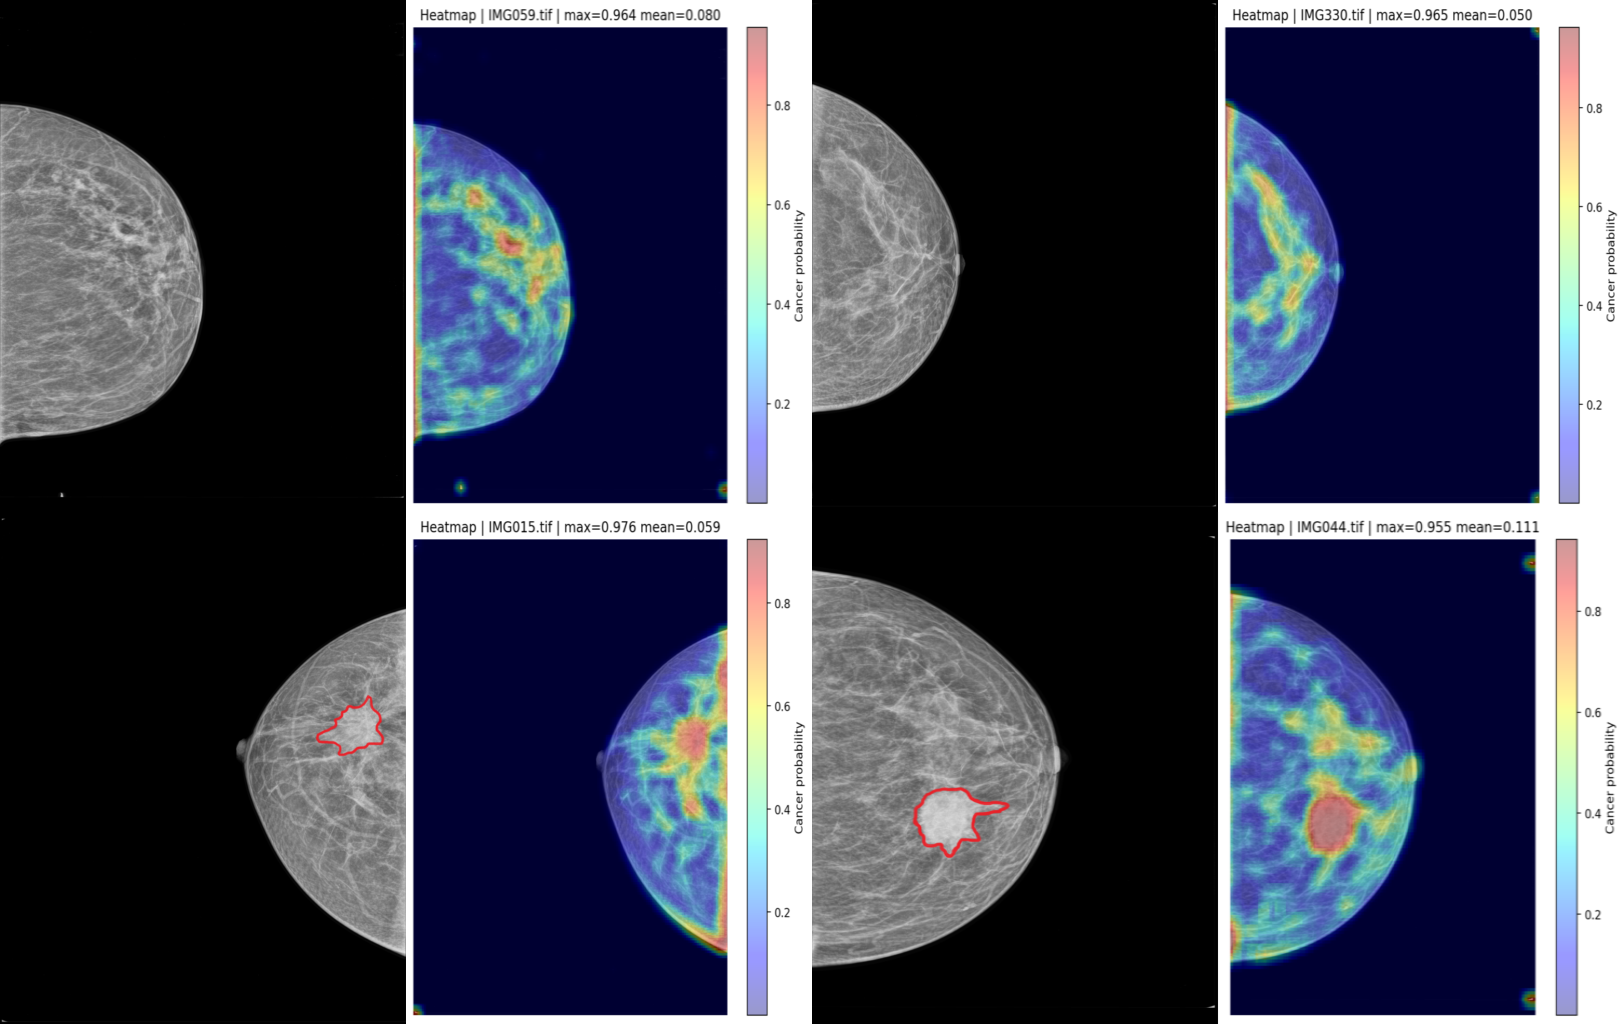
\includegraphics[width=0.95\linewidth]{../results/exp_022_mmr_n10_k3/heatmaps_side_by_side.png}
    \caption{Heatmaps for \texttt{exp\_022\_mmr\_n10\_k3}.}
\end{figure}

\section*{Composition experiments}
In this section, we explore two new runs with composite kernels using different kernel bank sizes.
We vary the number of kernels per family (n\_per\_family) to create banks of different sizes,
and select a number of kernels (n\_Composition) for composition of the final model. In both cases, we use AUC to weight the composite kernels. Also experimented with fisher weighting, but results were slightly worse. \\

Shared settings:
\begin{itemize}[leftmargin=0.5in]
    \item Selection method: MMR
    \item Model: Logistic
    \item weight\_method: AUC
    \item normalize: None
\end{itemize}


\begin{center}
\begin{tabular}{lcccccc}
\toprule
Run & n\_per\_family & n\_Composition & Val AUC & Test AUC & Test ACC \\
\midrule
exp\_022\_mmr\_nperFamily10\_nComposition25 & 10 & 65 & 0.9049 & 0.9096 & 0.8487 \\
exp\_022\_mmr\_nperFamily50\_nComposition125 & 50 & 325 & 0.9217 & 0.9260 & 0.8652 \\
\bottomrule
\end{tabular}
\end{center}

\begin{figure}[H]
    \centering
    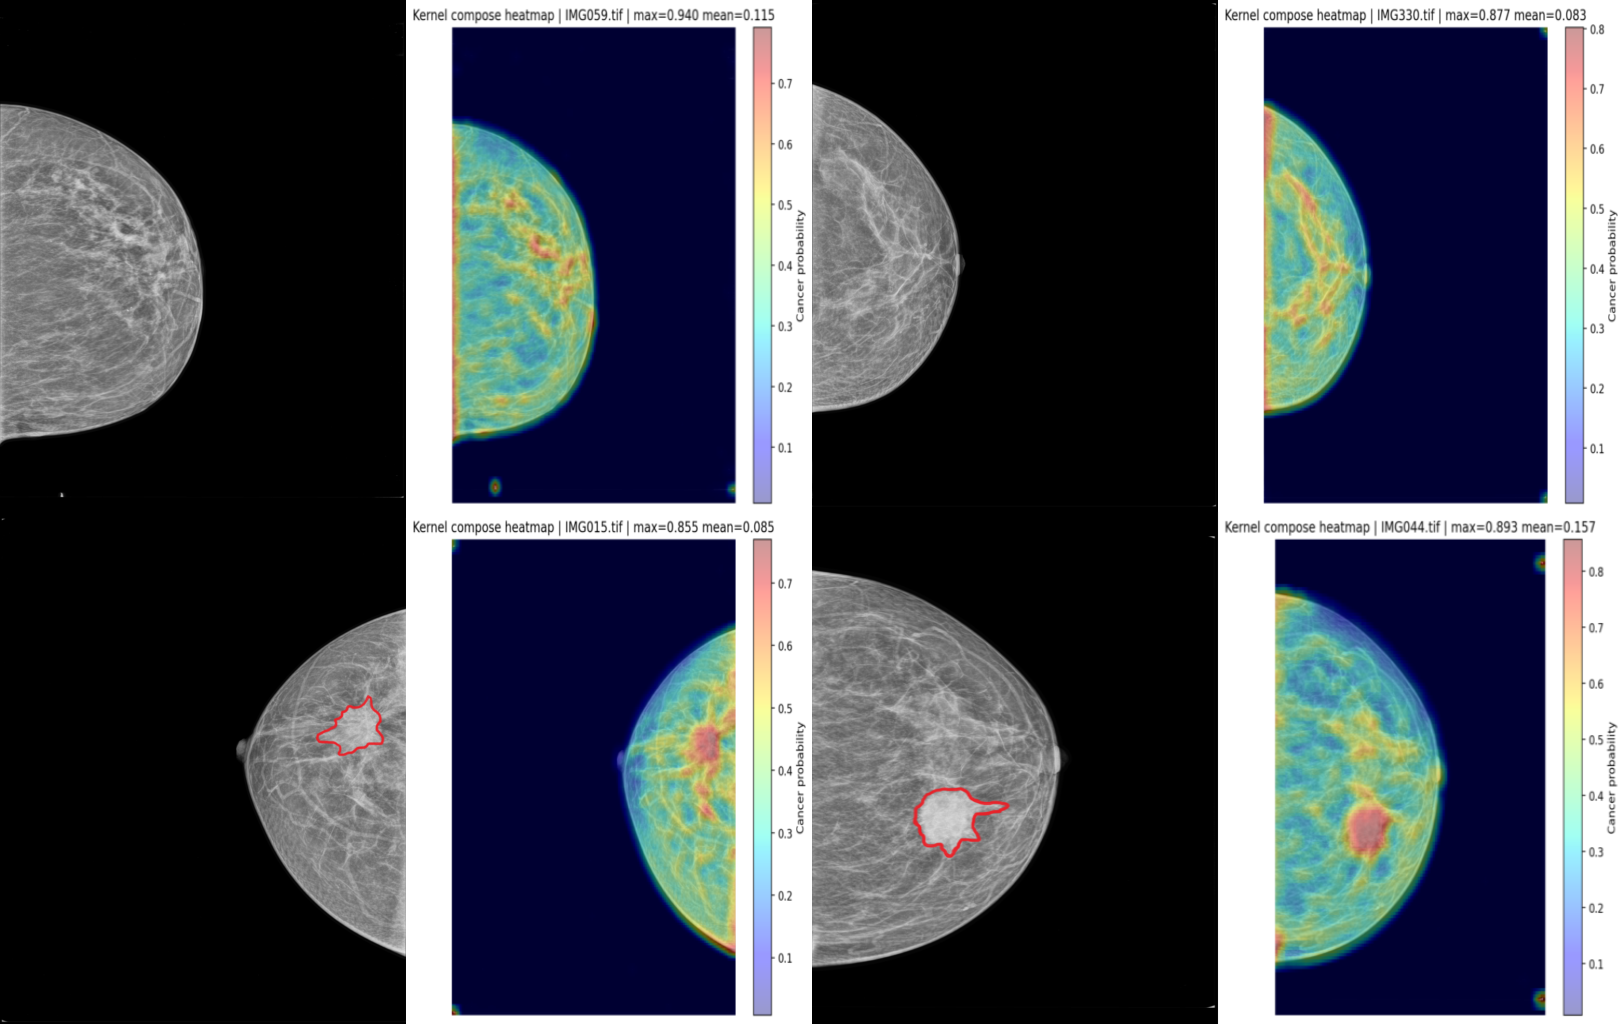
\includegraphics[width=0.95\linewidth]{../results/exp_022_mmr_nperFamily10_nComposition25/heatmaps_side_by_side.png}
    \caption{Composition heatmaps for exp\_022\_mmr\_nperFamily10\_nComposition25.}
\end{figure}
\begin{figure}[H]
    \centering
    
\includegraphics[width=0.95\linewidth]{../results/exp_022_mmr_nperFamily50_nComposition125/heatmaps_side_by_side.png}
    \caption{Composition heatmaps for exp\_022\_mmr\_nperFamily50\_nComposition125.}
\end{figure}

\paragraph{Conclusion}
The 125-composition run is the strongest of the new additions, exceeding the earlier baselines in both test AUC
(0.9260 vs 0.9239 for exp\_022\_mmr) and test accuracy (0.8652 vs 0.8182 for exp\_025\_mmr).
The 25-composition run is competitive but does not surpass the best baseline.

\end{document}
